\documentclass[12pt]{article}
\usepackage{xr}
\usepackage[a4paper, margin=1in]{geometry}
\usepackage{tikz}
\usetikzlibrary{positioning, arrows.meta, decorations.pathreplacing, calc, backgrounds,fit}
\usepackage{amsmath,amssymb}
\usepackage{mathrsfs} 
\usepackage{hyperref}
\usepackage{amsthm}
\usepackage{pdflscape} % For the landscape environment
\newtheorem{definition}{Definition}[section]
\newtheorem{remark}{Remark}[section]
\newtheorem{theorem}{Theorem}[section]
\newtheorem{axiom}{Axiom}[section]
\newtheorem{lemma}{Lemma}[section]
\newtheorem{proposition}{Proposition}[section]

\title{\textbf{Chapter 8: Analyzing the Testable Measurement}}
\author{Dmytro Surdu}
\begin{document}
\maketitle

\section{Prelude: Time‑Domains and Domain Ticks}
\label{sec:prelude-time}
At the very first glance at the non-trivial Testable Measurement, we observe that it necessarily maps multiple well-defined \textit{moments of time} associated with inputs \({z^{in}_1,\dots,z^{in}_n}\) to a \textit{single moment of time} when the basin \(\mathcal{B}\) is reached. Let's formalize this obviously \textit{behavioral} notion in the definition.

\subsection*{Discrete Time-Domains as First-Class Objects}

\begin{definition}[Discrete Time-Domain]
The \emph{discrete input time-domain} is the countable, well-ordered set
    \[
  \mathbb{T}_\mathfrak{D} \;=\; \{1,2,3,\dots\},
\] which indexes the distinct tuples \((q_i,t_i)\) named events, where \(q_i\) is generalized coordinates and \(t_i\) is time of the \(i\)-th event indexed by \(T_\mathfrak{D}\), supplied with the projection map \((q,t)\longrightarrow \mathbb{T}\) on the time space, so that events are identified by their times:
\[
\mathfrak{D} \;=\; \{d_1,d_2,\dots\}
\]
In a similar way, we define Discrete Space-Domain by using the projection map onto generalized coordinate space.
\end{definition}

\begin{definition}[External Input Time-Domain]
    The \textit{external input} time domain is is a Discrete Time-Domain which indexes the raw order in which the experimenter (or environment) supplies Testable Measurement inputs \(z^{\rm in}_t \in \mathcal Z^{\rm in}\).
\end{definition}
We will often omit the word \textit{external} if it is understood from the context.


\begin{definition}[Domain Tick]
An element \(d\in\mathbb T\) of any time-domain \(\mathfrak {D}\) will be called a \emph{domain tick}.  
\end{definition}


\subsection*{Why Time-Domains First?}

% TODO rewrite subsection completely. We have to narrate the deep profoundness of time domains. Particularly, their purely "behavioral" nature, which appears naturally due to the idea of adaptation, leads to the "anatomy" of the Testable Measurement described below. Decomposition requirements, on the contrary, will be relevant when introduced.

The Finite Tick‑0 decomposition and the Inductive (Shell‑by‑Shell) refinement both implicitly manipulate input ticks: they split, reorder, or loop over them.  Making \emph{time-domains explicit} is therefore the minimal and natural prelude to any systematic decomposition.  Multiplicity Perturbation provides the vocabulary for “why” we split; Response Promotion tells us “how” we repair the resulting guard-band violations.  The later normal-form theorems (finite guarded programs, loop-until entry, etc.) can thus be seen as canonical \emph{responses} to controlled time-domain multiplicity.

\section{Minimal Certification Standard \& Guard‑Bands}
\label{sec:min-standard-guardbands}

We fix a Testable Measurement
\[
  \mathfrak M=(\mathcal M,\mathcal Z^{\rm in},\mathcal Z^{\rm out},U,E)
\]
with compact metric spaces \(\mathcal M,\mathcal Z^{\rm in},\mathcal Z^{\rm out}\), continuous maps \(U,E\), and a reachable, invariant basin
\[
  \mathcal B \;=\; \{\Theta\in\mathcal M : L(\Theta)\le r\},
\]
defined by the Lyapunov–border function \(L:\mathcal M\to\mathbb R_{\ge0}\) (Chapter~5).

\subsection*{Definition of the Minimal Certification Standard}

\begin{definition}[Minimal Certification Standard]
\label{def:minimal-standard}
A \emph{Minimal Certification Standard} is a nonincreasing sequence of positive radii
\[
  \mathcal S=\{\varepsilon_n\}_{n\ge1},
  \qquad
  \varepsilon_{n+1}\le\varepsilon_n,\ \ \varepsilon_n\downarrow 0,
\]
such that, for every index \(n\), the “index‑\(n\)” certification procedure is robust to all perturbations of size at most \(\varepsilon_n\) that are admissible for certificates of length \(n\) and such that

\medskip
 each \(\varepsilon_n\) is the \emph{infimum} of radii satisfying the above robustness conjunction at index \(n\).  Equivalently, there is no strictly smaller \(\varepsilon'_n<\varepsilon_n\) for which soundness and completeness of the index‑\(n\) verification still hold for all admissible trajectories.
\end{definition}

\subsection*{Shells and Guard‑Bands}

\begin{definition}[Thickened Shells (State Guard‑Bands)]
\label{def:Bn}
For each \(n\ge1\) define the \(n\)-th thickened basin
\[
  \mathcal B_n \;:=\; \{\Theta'\in\mathcal M:\operatorname{dist}(\Theta',\mathcal B)\le \varepsilon_n\}.
\]
We call \(\mathcal B_n\) the \emph{state guard‑band} at index \(n\).
\end{definition}

\begin{definition}[Input Guard‑Band (preimage form)]
\label{def:input-gb}
For \(\Theta\in\mathcal M\) and \(n\ge1\), define
\[
  G^{\rm in}_n(\Theta)
  \;:=\;
  U(\Theta,\cdot)^{-1}\!\bigl(\mathcal B_n\bigr)
  \;=\;
  \{\,z^{\rm in}\in\mathcal Z^{\rm in}:U(\Theta,z^{\rm in})\in\mathcal B_n\,\}.
\]
\end{definition}

\begin{definition}[Output Guard‑Band]
\label{def:output-gb}
For \(\Theta\in\mathcal M\) and \(n\ge1\), set
\[
  G^{\rm out}_n(\Theta)
  \;:=\;
  \{\,z^{\rm out}\in\mathcal Z^{\rm out}:
      d\bigl(z^{\rm out},E(\Theta)\bigr)\le \varepsilon_n
   \}.
\]
(Equivalence with the other bands will be established later under mild regularity of \(E\).)
\end{definition}

\subsection*{Border Robustness via the Standard}

\begin{lemma}[Border Robustness]
\label{lem:border-robustness}
Let \(\mathcal S=\{\varepsilon_n\}\) be a \emph{Minimal Certification Standard}.  Then:
\begin{enumerate}
  \item \textbf{Nestedness:} \(\mathcal B_{n+1}\subseteq \mathcal B_n\) for all \(n\).
  \item \textbf{Absorption after entry:} If a trajectory enters \(\mathcal B\) at time \(\tau\), then for all \(n\ge\tau\), \(\Theta_n\in\mathcal B\subseteq\mathcal B_n\).
  \item \textbf{Tightness (Minimality):} No smaller radius \(\varepsilon'_n<\varepsilon_n\) preserves both forward robustness and completeness at index \(n\).  Equivalently, each \(\varepsilon_n\) is optimal.
  \item \textbf{Forward closure:} If \(\Theta\in\mathcal B_n\) and an admissible index‑\(n\) input \(z^{\rm in}\) is applied, then \(U(\Theta,z^{\rm in})\in\mathcal B_n\).
\end{enumerate}
\end{lemma}

\begin{proof}
(1) Since \(\varepsilon_{n+1}\le\varepsilon_n\), the inclusion \(\mathcal B_{n+1}\subseteq\mathcal B_n\) is immediate.

(2) Reachability gives \(\tau<\infty\) with \(\Theta_\tau\in\mathcal B\); invariance keeps \(\Theta_n\in\mathcal B\) for all \(n\ge\tau\).  Because \(\mathcal B\subseteq\mathcal B_n\), absorption follows.

(3) Suppose a strict \(\varepsilon'_n<\varepsilon_n\) still guarantees (a) invariance under all admissible perturbations at index \(n\) and (b) completeness.  Then the index‑\(n\) procedure would remain sound using \(\varepsilon'_n\), contradicting minimality.  Thus \(\varepsilon_n\) is tight.

(4) If \(U(\Theta,z^{\rm in})\notin\mathcal B_n\) for an admissible \(z^{\rm in}\), the allowed perturbation would break robustness at index \(n\), contradicting the definition of admissibility tied to \(\varepsilon_n\).  Hence \(U(\Theta,z^{\rm in})\in\mathcal B_n\).
\end{proof}

\begin{remark}
Lemma~\ref{lem:border-robustness} isolates the precise role of the Standard: it furnishes a nested, forward‑closed “buffer” around \(\mathcal B\) with no slack.  The guard‑bands for inputs and outputs are then induced by \(U\) and \(E\) as preimage and image tolerances of these shells; their equivalence (after basin entry) is proved in the next section.
\end{remark}

\section{Three Aspects \& Uniqueness}
\label{sec:three-aspects}

Having fixed a minimal Certification Standard $\mathcal S=\{\varepsilon_n\}$ and the induced guard–band families, we now show that every Testable Measurement \emph{necessarily} decomposes into three ontological aspects—\textbf{Observation}, \textbf{Adaptation}, and \textbf{Restitution}—and that this decomposition is \emph{unique up to guard‑band equivalence}.  

Intuitively (for a computer scientist or a system architect), $\mathcal S$ acts as a “double knife” that first separates admissible \emph{inputs} from forbidden ones (Observation vs.\ Adaptation) and then separates certified \emph{outputs/witnesses} from uncertified ones (Adaptation vs.\ Restitution).

Another intuitive view (for a physicist or a metrologist) is that the Adaptation is compared with the Certification Standard, which acts as a gauge. Therefore, \textit{precisely the Adaptation can be understood as a core act of measurement}.

\subsection*{Canonical Aspect Decomposition}

Recall the state shells $\mathcal B_n$ (Def.~\ref{def:Bn}) and input/out\-put guard‑bands (Defs.~\ref{def:input-gb}–\ref{def:output-gb}).  Let $\tau$ be the (finite) basin‑entry time of a trajectory; below we only consider $n\ge\tau$ (pre‑entry there is no certification yet).

\begin{definition}[Canonical Aspects at Index $n$]\label{def:canonical-aspects}
For $n\ge\tau$ define:
\begin{enumerate}
\item \textbf{Observation aspect}
\[
  \mathsf O_n(\Theta) \;:=\; G^{\rm in}_n(\Theta)
  \;=\; \{\,z^{\rm in}: U(\Theta,z^{\rm in})\in\mathcal B_n\,\}.
\]
It is the set of all inputs \emph{admissible} at index $n$ for state $\Theta$.

\item \textbf{Adaptation aspect}
\[
  \mathsf A(\Theta,z^{\rm in}) \;:=\; U(\Theta,z^{\rm in})
  \qquad\text{with domain } z^{\rm in}\in \mathsf O_n(\Theta).
\]
It is the (restricted) update map acting only on admissible inputs.

\item \textbf{Restitution aspect}
\[
  \mathsf R_n(\Theta) \;:=\; \bigl(E(\Theta),\; w_n(\Theta)\bigr),
\]
where $w_n(\Theta)$ is \emph{the} (polynomial‑size) witness data determined by the certification protocol at index $n$ (e.g. the capture pair $(T,\Theta_T)$ or its Type‑A surrogate).  In particular, the \emph{output guard‑band}
\[
  G^{\rm out}_n(\Theta) 
  = \{z^{\rm out}: d(z^{\rm out},E(\Theta))\le\varepsilon_n\}
\]
is the admissible image set for the emitted measurement result.
\end{enumerate}
We call $(\mathsf O_n,\mathsf A,\mathsf R_n)$ the \emph{canonical aspect triple} at index $n$.
\end{definition}

\begin{remark}
The dependence of $\mathsf O_n$ and $\mathsf R_n$ on $n$ reflects the tightening radii $\varepsilon_n$; $\mathsf A$ itself does not change with $n$ (the physics of $U$ is fixed), only its admissible domain does.  After entry, all $n\ge\tau$ are semantically interchangeable for certification—hence we may suppress $n$ when no confusion arises.
\end{remark}

\subsection*{Axioms for an Aspect Decomposition}

To state uniqueness, we formalize what it means for \emph{any} triple $(O,A,R)$ to be a valid aspect decomposition “at index $n$”.

\begin{definition}[Valid Aspect Triple at Index $n$]\label{def:valid-triple}
A triple $(O_n,A,R_n)$ is a \emph{valid aspect decomposition} at index $n\ge\tau$ if:
\begin{enumerate}
  \item \textbf{Observation soundness:}
        $z^{\rm in}\in O_n(\Theta)\;\Rightarrow\;A(\Theta,z^{\rm in})\in\mathcal B_n$.
  \item \textbf{Observation completeness:}
        For every $z^{\rm in}$ such that $U(\Theta,z^{\rm in})\in\mathcal B_n$, we have $z^{\rm in}\in O_n(\Theta)$.
  \item \textbf{Adaptation agreement:}
        $A(\Theta,z^{\rm in}) = U(\Theta,z^{\rm in})$ for all $z^{\rm in}\in O_n(\Theta)$.  (No hidden state dynamics).
  \item \textbf{Restitution soundness:}
        $R_n(\Theta)=(z^{\rm out},w)$ must satisfy $z^{\rm out}\in G^{\rm out}_n(\Theta)$ and $w$ must be a correct NP witness for $\Theta$ at index $n$.
  \item \textbf{Restitution completeness:}
        If $z^{\rm out}\in G^{\rm out}_n(\Theta)$ and a correct witness exists, then $R_n(\Theta)$ emits such a pair. 
\end{enumerate}
\end{definition}

Items (1)–(2) force $O_n$ to be \emph{exactly} the preimage of $\mathcal B_n$ under $U(\Theta,\cdot)$; (3) forbids hiding dynamics in “Observation” or “Restitution”.  Items (4)–(5) tie $R_n$ tightly to $E$ and the minimal standard (no slack in output tolerance or witness size).

\subsection*{Uniqueness Theorem}

\begin{theorem}[Three‑Aspect Uniqueness]\label{thm:aspect-uniqueness}
Let $\mathfrak M$ satisfy compactness, continuity, reachability, invariance, and let $\mathcal S$ be a minimal Certification Standard.  For each $n\ge\tau$ the canonical triple $(\mathsf O_n,\mathsf A,\mathsf R_n)$ (Def.~\ref{def:canonical-aspects}) is a valid aspect decomposition.  Moreover, if $(O_n,A,R_n)$ is any other valid triple (Def.~\ref{def:valid-triple}), then
\[
  O_n(\Theta) = \mathsf O_n(\Theta),\qquad
  A(\Theta,z^{\rm in}) = \mathsf A(\Theta,z^{\rm in}),\qquad
  R_n(\Theta)=\mathsf R_n(\Theta)
\]
for all $\Theta$ in the reachable set and all $z^{\rm in}\in O_n(\Theta)$.  Hence the decomposition is unique up to guard‑band equivalence.
\end{theorem}

\begin{proof}
\textbf{Existence.}  By construction $\mathsf O_n(\Theta)=G^{\rm in}_n(\Theta)$, and Lemma~\ref{lem:border-robustness}(4) gives Observation soundness.  Observation completeness follows from the definition of $G^{\rm in}_n$ as the full preimage.  $\mathsf A=U$ on its domain; Restitution soundness/completeness follow from minimality of $\mathcal S$ and the definition of $G^{\rm out}_n$ (any smaller image set or witness would violate tightness).  Thus the canonical triple is valid.

\smallskip
\textbf{Uniqueness of $O_n$.}  
Suppose there exists $z^{\rm in}$ with $U(\Theta,z^{\rm in})\in\mathcal B_n$ but $z^{\rm in}\notin O_n(\Theta)$.  Then Observation completeness (Def.~\ref{def:valid-triple}.2) fails.  Conversely, if $z^{\rm in}\in O_n(\Theta)$ but $U(\Theta,z^{\rm in})\notin\mathcal B_n$, Observation soundness (1) fails.  Hence $O_n(\Theta)$ must coincide with the full preimage $G^{\rm in}_n(\Theta)=\mathsf O_n(\Theta)$.

\smallskip
\textbf{Uniqueness of $A$.}  
By (3), $A(\Theta,z^{\rm in})$ must equal $U(\Theta,z^{\rm in})$ on the domain $O_n(\Theta)$, so $A=\mathsf A$ there.  Any deviation would either hide dynamics in Observation (violating (3)) or push the image outside $\mathcal B_n$ (violating (1)), or permit a smaller $\varepsilon_n$ (contradicting minimality).

\smallskip
\textbf{Uniqueness of $R_n$.}  
Assume $R_n(\Theta)=(z^{\rm out},w)$ differs from the canonical $\mathsf R_n(\Theta)=(E(\Theta),w_n(\Theta))$ on the reachable set.  If $z^{\rm out}\notin G^{\rm out}_n(\Theta)$, Restitution soundness (4) fails.  If $z^{\rm out}$ is inside but differs while still maintaining correctness, then—because $E$ is continuous and $\varepsilon_n$ is tight—one could shrink $\varepsilon_n$ slightly and keep soundness/completeness, contradicting minimality.  Similarly, if $w$ is shorter or weaker than the canonical witness, minimality of the witness size (implied by minimal $\varepsilon_n$ together with polynomial bound) would be contradicted.  Therefore $R_n=\mathsf R_n$.

\smallskip
\textbf{Guard‑band equivalence.}  
All equalities above hold on the reachable set and for inputs inside the admissible bands.  On the (closed) guard‑band boundaries different triples could disagree without affecting certification; we declare those discrepancies \emph{guard‑band equivalent}.  Thus uniqueness holds “up to guard‑band equivalence.”
\end{proof}

\begin{remark}
The proof shows that uniqueness is ultimately a corollary of \emph{minimality}: if any aspect were “looser” or “tighter” than the canonical one, we could shrink or enlarge $\varepsilon_n$ and still certify, contradicting that $\varepsilon_n$ is the infimum.  Hence the three cuts enforced by $\mathcal S$ are logically determined and not a matter of design choice.
\end{remark}

\section{Singular Certified Result and the Simple Test}
\label{sec:singular-result-simple-test}

The three–aspect decomposition fixes \emph{how} a Testable Measurement certifies.  We now isolate \emph{what} is ultimately certified.  The key point is a \emph{singularity}: modulo guard‑band equivalence, there is only one epistemically non‑redundant certified outcome.  This motivates the notion of a \emph{Simple Test}.

\subsection*{The First Certified Tick is Epistemically Maximal}

Let $\tau$ be the (finite) basin–entry time and recall that for $n\ge\tau$ the canonical aspects $(\mathsf O_n,\mathsf A,\mathsf R_n)$ are well‑defined.  Define the \emph{first certified emission}
\[
  \bigl(z^{\rm out}_\tau,\; w_\tau\bigr)
  \;:=\; \mathsf R_\tau(\Theta_\tau)
  \;=\;\bigl(E(\Theta_\tau),\;w_\tau(\Theta_\tau)\bigr).
\]

\begin{proposition}[Singularity of the Certified Result]
\label{prop:singularity}
For every $n>\tau$,
\[
  \mathsf R_n(\Theta_n)
  \quad\text{is guard-band equivalent to}\quad
  \mathsf R_\tau(\Theta_\tau).
\]
In particular, any later certified output carries no new certifiable information about the tail predicate beyond what was already established at $t=\tau$.
\end{proposition}

\begin{proof}
By invariance, $\Theta_n\in\mathcal B$ for $n\ge\tau$.  By Lemma~\ref{lem:border-robustness}(1) and (2), $\mathcal B\subseteq\mathcal B_n$ and $\varepsilon_n\le\varepsilon_\tau$.  Hence $d\bigl(E(\Theta_n),E(\Theta_\tau)\bigr)\le\varepsilon_\tau$ implies both outputs lie inside $G^{\rm out}_\tau(\Theta_\tau)$.  Minimality of $\varepsilon_\tau$ forbids shrinking the tolerance without breaking robustness, so any difference between $E(\Theta_n)$ and $E(\Theta_\tau)$ is within the unavoidable guard-band.  The same argument applies to witnesses: if a “shorter” or “different” $w_n$ existed, minimality of the index‑$\tau$ witness would be contradicted.  Thus all later restitutions are equivalent up to the guard-band defined at $\tau$.
\end{proof}

\subsection{Singular Time-Domain definition}

Because the Testable Measurement first certified tick carries all distinguishable information about the measurement result, it is worth to underscore its singularity on the definition.

\begin{definition}[Singular Time-Domain]
A \emph{Singular Time-Domain} is the singleton set
\[
  \mathbb T_{\Sigma} \;=\; \{\mathcal d\},
\]
used to model a \emph{Simple Test}: all certified behaviour is represented by one effective tick.  Equivalently, all post-entry evolution is epistemically collapsed into \(\mathcal d\).
\end{definition}

\subsection*{Certified Indices and Collapse Maps}

\begin{definition}[Certified Index Set and Collapse Map]
Let \(\tau\) be the (finite) basin-entry time.  Define the \emph{certified index set}
\[
  \mathbb N_{\mathrm{cert}}=\{1,2,3,\dots\},
\]
and a partial map \(\pi:\mathbb T_{\mathrm{ext}}\to\mathbb N_{\mathrm{cert}}\) by
\[
  \pi(t)=
  \begin{cases}
    \text{undefined}, & t<\tau,\\[2pt]
    1, & t=\tau,\\[2pt]
    f(t), & t>\tau,
  \end{cases}
\]
where \(f\) records any (possible) further certified emissions.  In a Simple Test,
\(\pi(t)=1\) for all \(t\ge\tau\).  The induced equivalence relation
\(t\sim t'\iff \pi(t)=\pi(t')\) collapses the raw timeline onto the certified one.
\end{definition}

\begin{remark}[Singular Collapse]
When \(\pi(t)=1\) for all \(t\ge\tau\), all post-entry ticks coalesce into a single certified tick.  This is the \emph{Singular Time-Domain} phenomenon and characterizes the Simple Test.
\end{remark}

% 

\subsection*{Definition of the Simple Test}

\begin{definition}[Simple Test]
\label{def:simple-test}
A Testable Measurement is a \emph{Simple Test} if, after basin entry at time $\tau$, it produces no further distinct certified emissions.  Formally, the collapse map $\pi:\mathbb T_{\mathrm{ext}}\to\mathbb N_{\mathrm{cert}}$ satisfies
\[
  \pi(t)=1\qquad\forall t\ge\tau.
\]
Equivalently, the certified time-domain is the \emph{Singular Time-Domain}
\[
  \mathbb T_\Sigma=\{1\}
  \;\cong\;
  \{\tau,\tau+1,\tau+2,\dots\}/\sim,
\]
where all post-entry ticks are identified.
\end{definition}

\begin{remark}[Maximal Compression]
Among all non-trivial certifiable measurements, the Simple Test realizes \emph{maximal index collapse}: no pre-entry tick can be merged with the post-entry class without violating soundness, and all post-entry ticks are epistemically indistinguishable.  A diagram of the \emph{double split} (Observation/Adaptation/Restitution) placed here visually ties this singularity to the Certification Standard’s two cuts.
\end{remark}

\begin{landscape}
\begin{figure}[ht!]
  \centering
  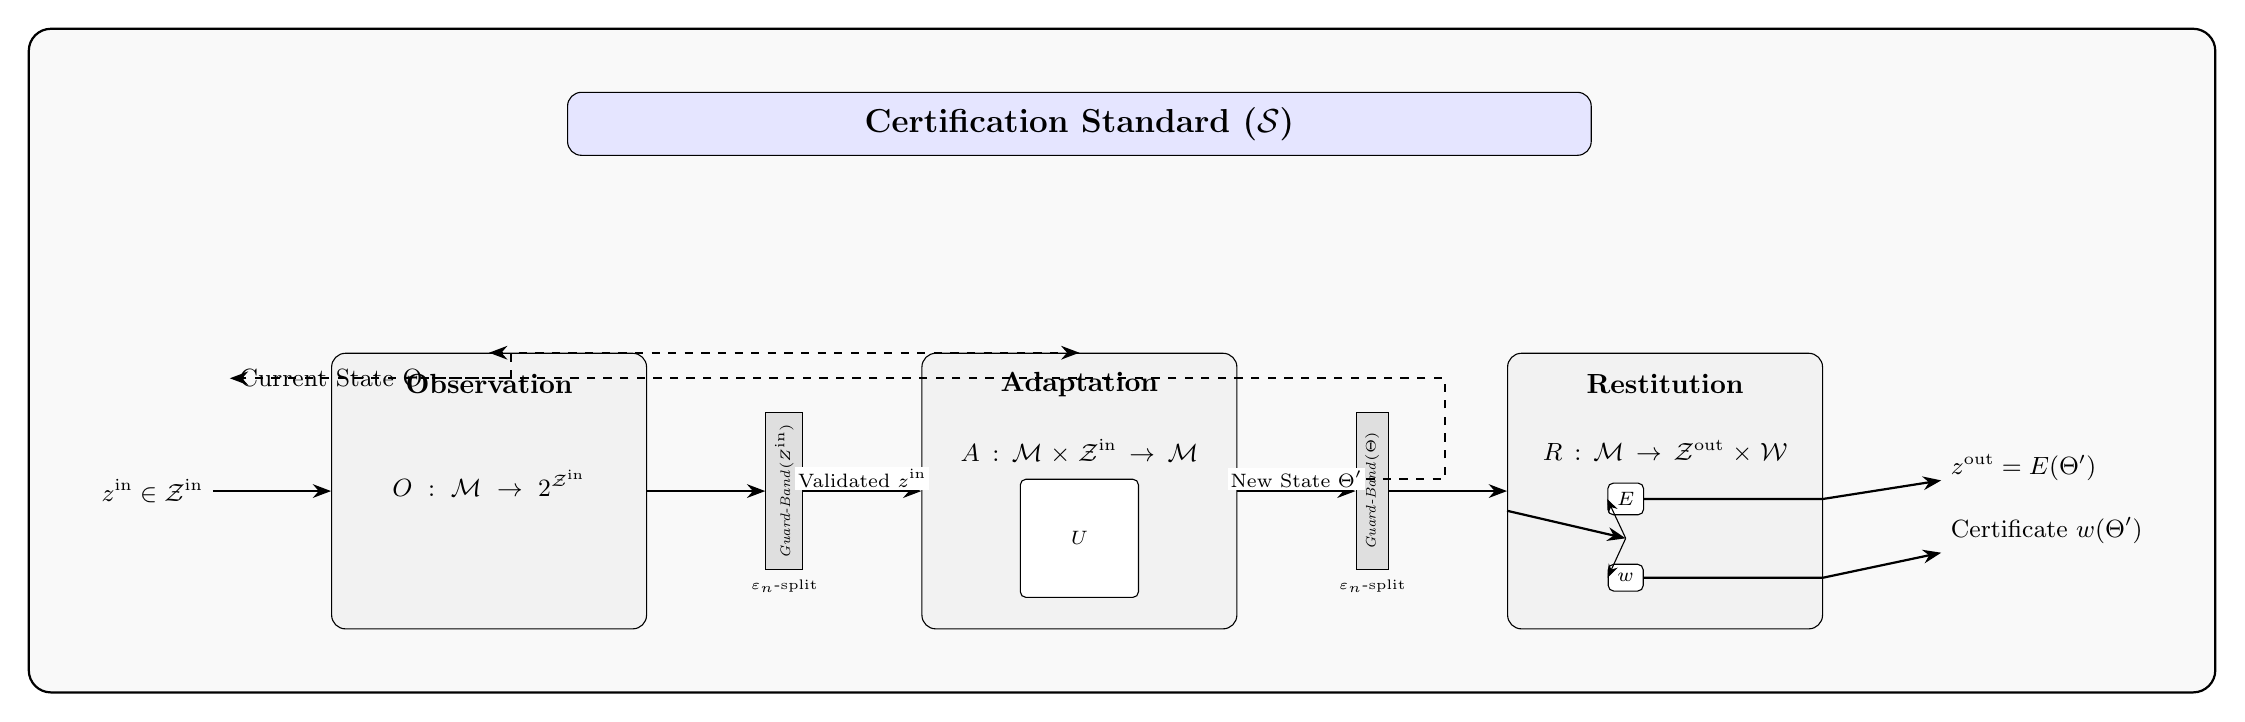
\begin{tikzpicture}[
    auto,
    >=Stealth,
    node distance=0.8cm and 1.5cm,
    % Styles
    aspect/.style={
        draw, rectangle, rounded corners=5pt,
        minimum width=4cm, minimum height=3.5cm,
        align=center, fill=gray!10,
        font=\small
    },
    io/.style={font=\small},
    func/.style={
        draw, rectangle, fill=white,
        font=\scriptsize\ttfamily, rounded corners=2pt,
        align=center
    },
    label/.style={font=\bfseries},
    arrowlabel/.style={font=\scriptsize, midway, fill=white, inner sep=1pt, align=center},
    mathlabel/.style={font=\small, text width=4cm, align=center},
    standard/.style={
        draw, rounded corners=5pt, fill=blue!10,
        font=\large\bfseries, align=center,
        minimum width=13cm, minimum height=0.8cm
    },
    guard_band_split/.style={
        draw, fill=gray!25, minimum height=2cm, minimum width=0.4cm,
        align=center, font=\tiny
    },
    background_block/.style={
        draw, thick, rounded corners=8pt, fill=gray!5,
        inner sep=0.8cm
    }
  ]

    % --- Define primary components first ---
    \node (Obs) [aspect] {};
    \node (GB1) [guard_band_split, right=of Obs] {\rotatebox{90}{\textit{Guard-Band}($Z^{\text{in}}$)}};
    \node (Ad)  [aspect, right=of GB1] {};
    \node (GB2) [guard_band_split, right=of Ad] {\rotatebox{90}{\textit{Guard-Band}($\Theta$)}};
    \node (Res) [aspect, right=of GB2] {};

    % --- Place Certification Standard at the very top ---
    \node (Standard) [standard, above=2.5cm of Ad] {Certification Standard ($\mathcal{S}$)};

    % --- Populate the Aspect Boxes ---
    \node[label] at (Obs.north) [yshift=-0.4cm] {Observation};
    \node[mathlabel] at (Obs.center) [yshift=0.1cm] {$O : \mathcal M \rightarrow 2^{\mathcal Z^{\rm in}}$};
    \node[label] at (Ad.north) [yshift=-0.4cm] {Adaptation};
    \node[mathlabel] at (Ad.center) [yshift=0.5cm] {$A : \mathcal M \times \mathcal Z^{\rm in} \rightarrow \mathcal M$};
    \node (update) [func, minimum size=1.5cm] at (Ad.center) [yshift=-0.6cm] {$U$};
    \node[label] at (Res.north) [yshift=-0.4cm] {Restitution};
    \node[mathlabel] at (Res.center) [yshift=0.5cm] {$R : \mathcal M \rightarrow \mathcal Z^{\rm out} \times \mathcal W$};
    \coordinate (split_point) at ($(Res.center) + (-0.5cm, -0.6cm)$);
    \node (eval) [func] at (split_point) [yshift=0.5cm] {$E$};
    \node (wit)  [func] at (split_point) [yshift=-0.5cm] {$w$};

    % --- Inputs and Outputs ---
    \node (zin) [io, left=of Obs] {$z^{\rm in} \in \mathcal Z^{\rm in}$};
    \node (theta_current) [io, above=1.2cm of Obs.west] {Current State $\Theta$};
    \node (zout) [io, right=of Res.east, yshift=0.3cm] {$z^{\rm out} = E(\Theta')$};
    \node (wout) [io, right=of Res.east, yshift=-0.5cm] {Certificate $w(\Theta')$};

    % --- Main left-to-right flow ---
    \draw[->, thick] (zin) -- (Obs);
    \draw[->, thick] (Obs.east) -- (GB1.west);
    \draw[->, thick] (GB1.east) -- (Ad.west) node[arrowlabel] {Validated $z^{\rm in}$};
    \draw[->, thick] (Ad.east) -- (GB2.west) node[arrowlabel] (theta_prime_arrow) {New State $\Theta'$};
    \draw[->, thick] (GB2.east) -- (Res.west);

    % --- Restitution internal flow ---
    \draw[->, thick] ($(Res.west)+(0, -0.25cm)$) -- (split_point);
    \draw[->] (split_point) -- (eval.west);
    \draw[->] (split_point) -- (wit.west);
    \draw[->, thick] (eval.east) -- (eval.east -| Res.east) -- (zout);
    \draw[->, thick] (wit.east) -- (wit.east -| Res.east) -- (wout);

    % --- Clean State Distribution and Feedback Loop ---
    \coordinate (dist_path) at ($(theta_current.east) + (1cm, 0)$);
    \draw[thick, dashed] (theta_current.east) -- (dist_path);
    \draw[->, thick, dashed] (dist_path) |- (Obs.north);
    \draw[->, thick, dashed] (dist_path) |- (Ad.north);
    
    \draw[->, thick, dashed] (theta_prime_arrow.east) -- ++(1,0) |- (theta_current.west);
        
    % --- Guard band split labels ---
    \node[font=\tiny] at (GB1.south) [yshift=-0.2cm] {$\varepsilon_n$-split};
    \node[font=\tiny] at (GB2.south) [yshift=-0.2cm] {$\varepsilon_n$-split};
    
    % --- Background Block ---
    \begin{pgfonlayer}{background}
        \node [
            background_block,
            fit=(Standard) (zin) (zout) (wout) (theta_current) (Res.south),
            label={[font=\bfseries, anchor=south, yshift=0.2cm]north:Testable Measurement \(\mathfrak{M}\)}
        ] {};
    \end{pgfonlayer}

  \end{tikzpicture}
  \caption{
      The Certification Standard ($\mathcal{S}$) acts as an active, double-splitting “knife,” forcing a decomposition of the measurement process into three fundamental aspects. Alternatively, it can be viewed as a gauge for the core act of the measurement - the Adaptation. Each conceptual “cut” is wrapped by a guard-band $\varepsilon_n$. The resulting aspects are: \textbf{Observation} (accepting inputs), \textbf{Adaptation} (updating the internal state), and \textbf{Restitution} (producing a certified result and witness). This structure is not a design choice but a necessary consequence of building a Testable Measurement $\mathfrak{M}$. The process is inherently stateful: the new state $\Theta'$ becomes the current state $\Theta$ for the next iteration, as shown by the feedback loop.
  }
\end{figure}
\end{landscape}

\section{Conclusion}
What we have been doing in this Chapter is:
\begin{enumerate}
  \item \textbf{Introducing Time-Domains.}  
        Observing the event map collapse, we complemented the \textit{output} Singular Time-Domain of the Simple Test by an explicit and, generally, multi-tick \textit{input} time-domain. 
  \item \textbf{Exhibiting the Minimal Certification Standard.}  
        The standard $\mathcal S=\{\varepsilon_n\}$ is not an add-on; it \emph{induces} state, input, and output guard-bands. It is the “knife” that slices the measurement into Observation, Adaptation, and Restitution.
  \item \textbf{Proving Three-Aspects Uniqueness and the Simple Test.}  
        Once $\mathcal S$ is in place, the three aspects are forced and unique (up to null sets). The Simple Test emerges as the canonical form: one certified tick, maximal index collapse, Singular Time-Domain.
\end{enumerate}
\subsection{What are our takes from this?}
\begin{itemize}
    \item We got a clear understanding of how the Testable Measurement behaves. Due to the behavior, its best name is Simple Test: a piece of work which yields a single distinguishable result. The work starts from more events filled with information, but this multiplicity inevitably collapses to a single output event.
    \item We also got a clear picture of the Simple Test "anatomy". The Certification Standard induces the equivalent post-entry state and input guard bands; it splits the process into three canonical parts - Observation, Adaptation, and Restitution. 
    
    Unlike many works where these aspects were introduced ad hoc, here we can see the explicit cause of their existence: Certification Standard is a gauge against which we check our measurement model representation, build in Adaptation. 
    
    Therefore, we can identify Adaptation as a core part of a measurement, while Observation and Restitution are its "interfaces" with well-defined (by guard bands) contracts.
\end{itemize}

\subsection{What's next?}

The obtained results are ontologically rich, because everything is obtained from the first principle. However, they don't seem to be very helpful if we design a system constructively. So far, we have recovered some core concepts and objects in metrology; that's all.

The immediate question is: can we decompose a Simple Test further?

To answer this question, let's recall we observed a multi-tick input time-domain. It was already present by a map collapse; so nothing is introduced ad hoc here. 

But in the next chapter, we will see that the result of reviewing this structure closely is decisive: without distinct input ticks, there is no space to decompose, schedule, or control anything.

\end{document}